The dataset \cite{dataset} includes the unit sales of 3,049 products sold by Walmart in the USA in grouped time-series format. 
The products are classified in three categories (Hobbies, Foods, and Household) and seven departments. 
Additionally, these products are sold across ten stores, located in the three states of California (CA), Texas (TX), and Wisconsin (WI). Specifically, there are four stores located in California, three in Texas, and three in Wisconsin.
The dataset contains the following three data files \cite{m5}:
\begin{itemize}
    \item \textbf{calendar.csv}: contains information about the dates the products were sold, such as promotions, holidays, and other events.
    \item \textbf{sell\_prices.csv}: contains the average weekly price of each item.
    \item \textbf{sales\_train.csv}: contains the daily unit sales of each item.
\end{itemize}

\begin{wrapfigure}{r}{0.46\textwidth}
    \vspace{-25pt}
    \centering
    \captionsetup{width=.46\textwidth}
    \fbox{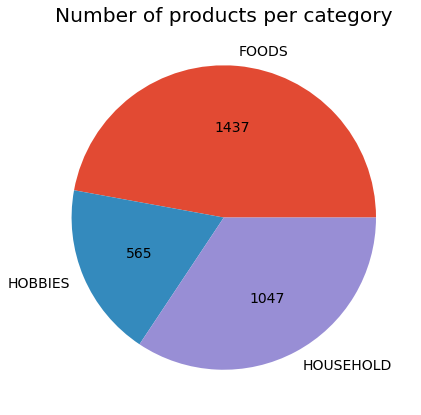
\includegraphics[width=0.42\textwidth]{figures/exploratory_data_analysis/item_cats.png}}
    \caption{Number of products per category.}
    \label{fig:item_cats}
    \vspace{-20pt}
\end{wrapfigure}

Figure \ref{fig:item_cats} shows the number of products per category. 
There are 1437, 1047, and 565 products in the \texttt{Foods}, \texttt{Household}, and \texttt{Hobbies} categories, respectively, for a total of 3049 products. 
Since these products are sold across ten different stores, there is a total of 30,490 items, out of which 22,243 had a price change at some point in time. 
In addition, from Figure \ref{fig:price_all}, which shows the price distribution of all products, we can see that most items cost between three to four dollars.
Furthermore, Figure \ref{fig:price_cats} shows the price distribution of each product category separately.
It is apparent that the \texttt{Hobbies} products do not have the same price distribution as \texttt{Foods} and \texttt{Household} products and tend to have more products that are very cheap.

\begin{figure}[b!]
    \centering
    \captionsetup{width=.93\textwidth}
    \fbox{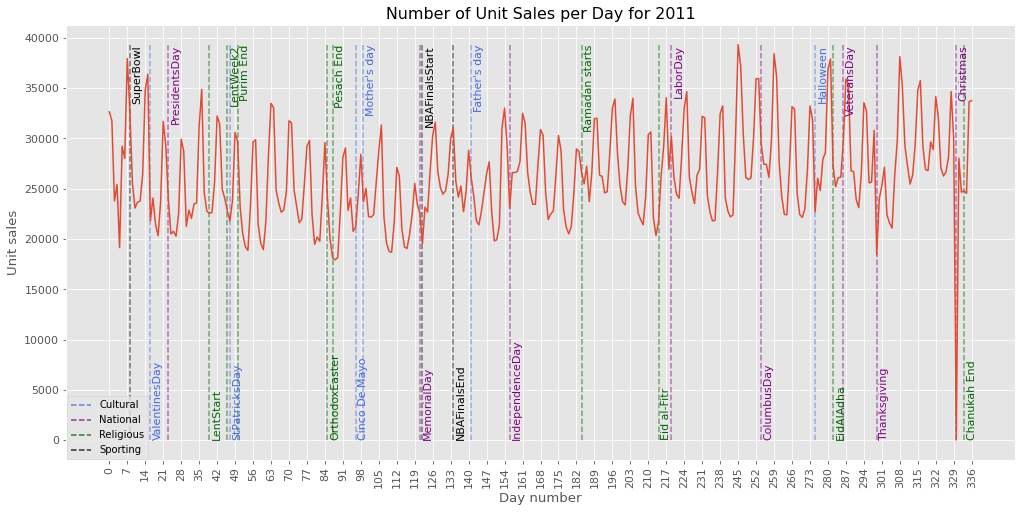
\includegraphics[width=0.93\textwidth]{figures/exploratory_data_analysis/daily_sales_2011.png}}
    \caption{The number of unit sales per day in 2011.}
    \label{fig:daily_sales_2011}
\end{figure}

\begin{figure}[t]
    \centering
    \captionsetup{width=.93\textwidth}
    \fbox{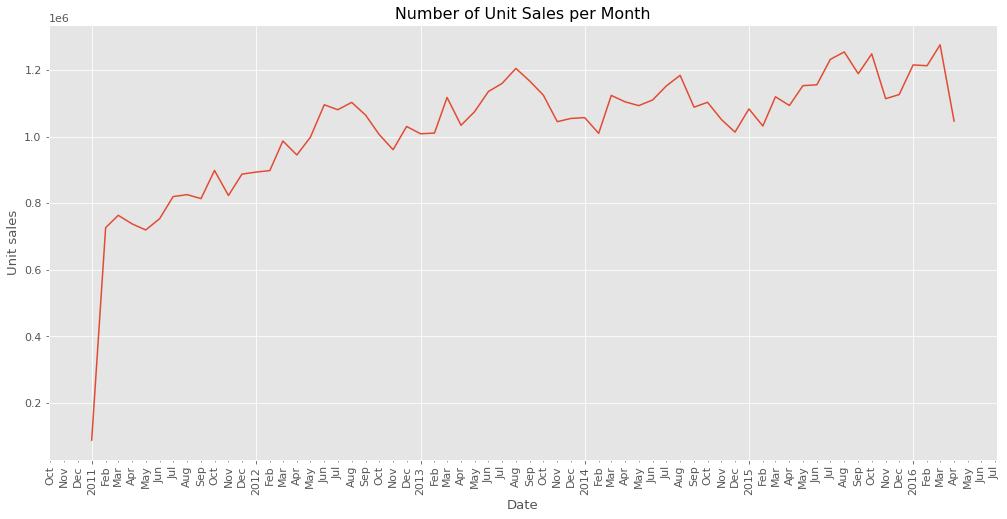
\includegraphics[width=0.93\textwidth]{figures/exploratory_data_analysis/monthly_sales.png}}
    \caption{The number of unit sales per month.}
    \label{fig:monthly_sales}
    \vspace{-2.5mm}
\end{figure}

On another point, Figure \ref{fig:ma_4week} shows a 4-week moving-average of the revenue earned, number of units sold, and the average price of all items.
We see that the average price of products are increasing over time in a linear fashion. Moreover, as expected, revenue and unit sales have increased with almost an identical pattern. Additionally, examining the revenue and unit sales graphs, we can see some form of seasonality in the curves.
Hence, we further explore for any seasonality patterns. From Figure \ref{fig:daily_sales_2011}, which shows the number of unit sales per day for the year 2011, we see a clear weekly pattern in the number of unit sales.
Specifically, the number of units sold tends be the highest during the weekends and the lowest in the middle of the week. 
This can be confirmed by examining Figure \ref{fig:dow_sales}, which shows the average number of units sold per day of week for all years.
Additionally, Figure \ref{fig:daily_sales_2011} shows national holidays and other special events, which are considered as external factors and may affect the number of unit sales. 
Most national holiday events, such as Thanksgiving, have a negative effect on the number of unit sales, possibly because people tend to spend time with their families rather than shopping. 
Additionally, Figure \ref{fig:monthly_sales} shows the number of unit sales per month, which shows that the number of sales tend to increase as we approach the middle of the year and falls off at the end of the year.
Moreover, we can see a spike in sales during March.
This is confirmed by examining Figure \ref{fig:moy_sales}, which shows the average number of units sold in each month of the year. 

\begin{figure}[H]
    \begin{minipage}{0.48\textwidth}
        \centering
        \vspace{3mm}
        \captionsetup{width=.98\textwidth}
        \fbox{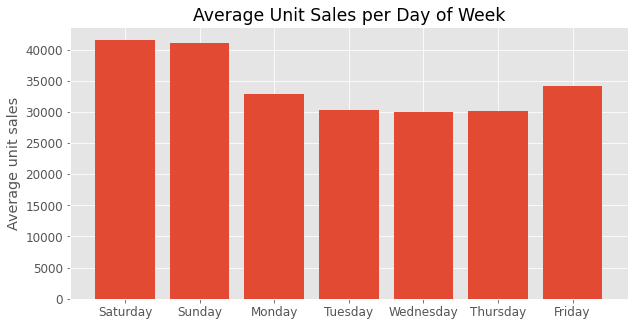
\includegraphics[width=0.98\textwidth]{figures/exploratory_data_analysis/dow_sales.png}}
        \caption{Average number of units sold per day of week.}
        \label{fig:dow_sales}
    \end{minipage}
    \hfill
    \begin{minipage}{0.48\textwidth}
        \centering
        \captionsetup{width=.98\textwidth}
        \fbox{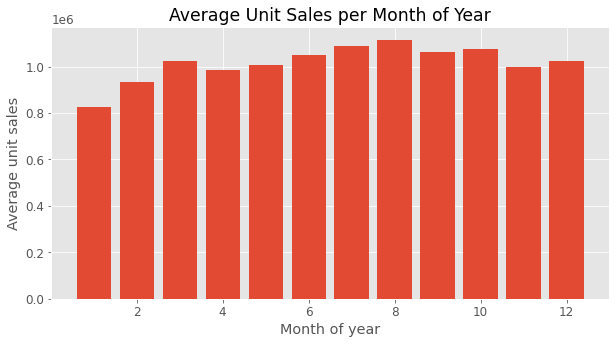
\includegraphics[width=0.98\textwidth]{figures/exploratory_data_analysis/moy_sales.png}}
        \caption{Average number of units sold per month.}
        \label{fig:moy_sales}
    \end{minipage}
\end{figure}

In the rest of this chapter, we will group the items based on their categories, states, stores, and departments and compare their sales data.

\section{Product Categories}
\begin{wrapfigure}{r}{0.55\textwidth}
    \vspace{-15pt}
    \centering
    \captionsetup{width=0.52\textwidth}
    \fbox{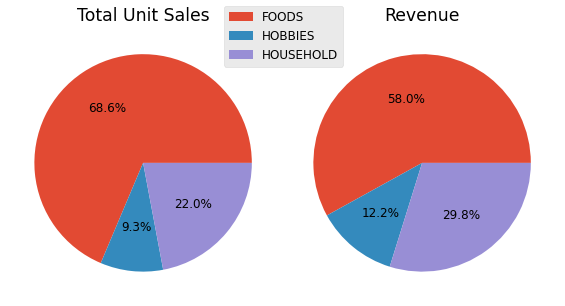
\includegraphics[width=0.52\textwidth]{figures/exploratory_data_analysis/sales_rev_cats.png}}
    \caption{Proportion of units sold and revenue earned in each product category.}
    \label{fig:sales_rev_cats}
    \vspace{-20pt}
\end{wrapfigure}
   
Furthermore, we examine the number of units sold and revenue earned from each product category.
By examining the pie charts in Figure \ref{fig:sales_rev_cats}, we see that the \texttt{Foods} category accounts for most of the units sold and revenue earned, with 68.6\% of all products sold belonging to the \texttt{Foods} category, which corresponds to 58.0\% of the total revenue earned.
Moreover, figure \ref{fig:cat_sales} shows a time-series of the number of unit sales per category.
It is apparent that the \texttt{Foods} category has a lot more sales that the other two categories.
Moreover, the sales for the \texttt{Foods} category seem to have a lot of oscillations that is less present in the other two categories.

\begin{figure}[b!]
    \centering
    \captionsetup{width=0.98\textwidth}
    \fbox{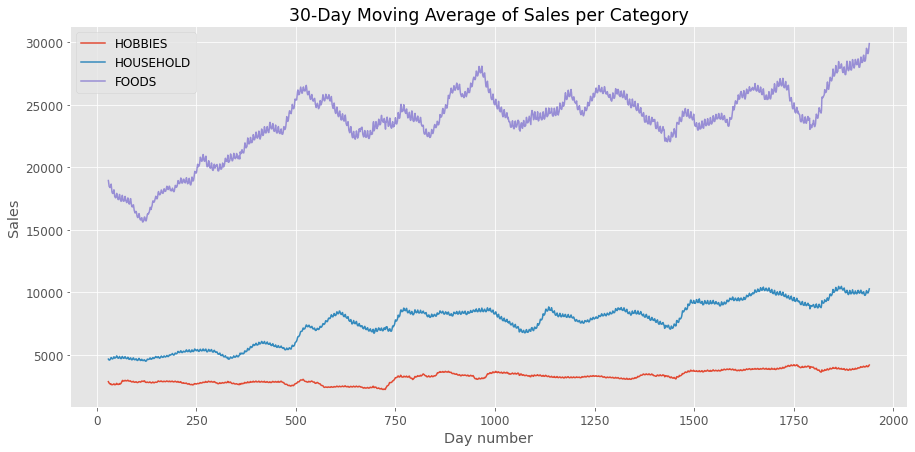
\includegraphics[width=0.98\textwidth]{figures/exploratory_data_analysis/cat_sales.png}}
    \caption{30-day moving average of sales per category.}
    \label{fig:cat_sales}
\end{figure} 


\section{States}
\begin{wrapfigure}{r}{0.55\textwidth}
    \vspace{-10pt}
    \centering
    \captionsetup{width=0.52\textwidth}
    \fbox{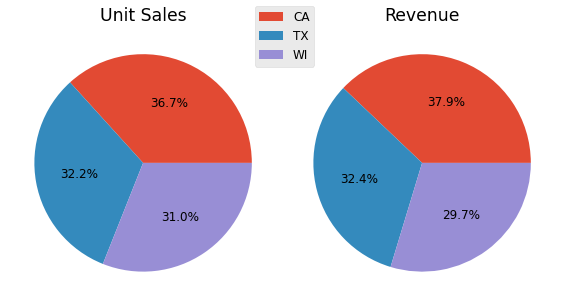
\includegraphics[width=0.52\textwidth]{figures/exploratory_data_analysis/sales_rev_states.png}}
    \caption{Proportion of units sold and revenue earned in each state.}
    \label{fig:sales_rev_states}
    \vspace{-20pt}
\end{wrapfigure}

Another factor to examine is whether there is any difference in the number of units sold and revenue earned between various states.
Figure \ref{fig:sales_rev_states} compares the total unit sales and revenue earned in each state. 
Since the number of stores is not constant between the states, the values for each state have been normalized by the number of stores in that state.
By examining the pie charts we see that, on average, the three states have about the same number of unit sales and revenue earned per store, however, the store in state of California are, on average, performing slightly better compared to the stores in Texas and Wisconsin. 
Furthermore, Figure \ref{fig:state_sales} shows that the state California has more oscillations in its sales compared to the other states.
\begin{figure}[H]
    \centering
    \captionsetup{width=0.98\textwidth}
    \fbox{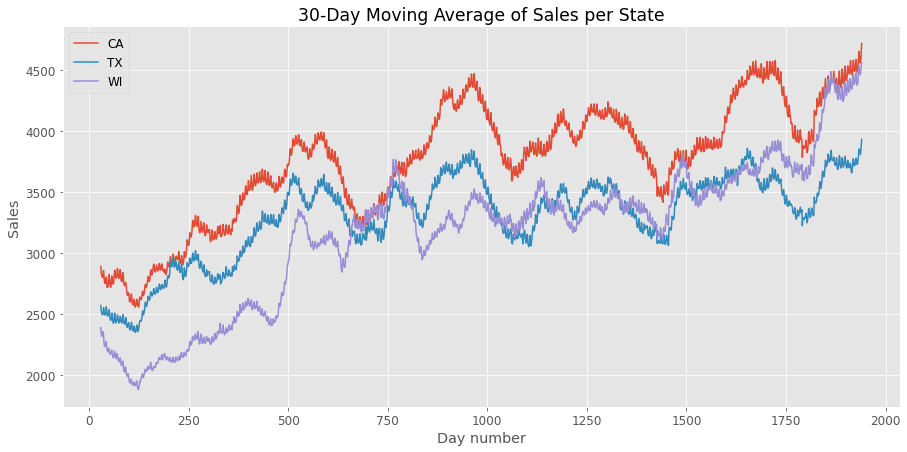
\includegraphics[width=0.98\textwidth]{figures/exploratory_data_analysis/state_sales.png}}
    \caption{30-day moving average of sales per state.}
    \label{fig:state_sales}
\end{figure} 


\section{Stores}
\begin{wrapfigure}{r}{0.55\textwidth}
    \vspace{-15pt}
    \centering
    \captionsetup{width=0.52\textwidth}
    \fbox{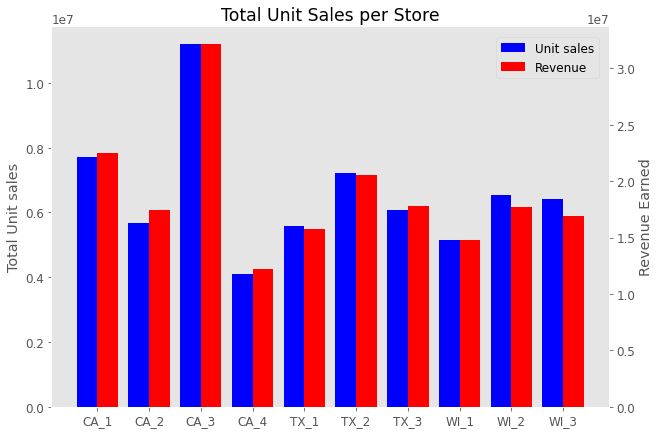
\includegraphics[width=0.52\textwidth]{figures/exploratory_data_analysis/sales_rev_stores.png}}
    \caption{Proportion of units sold and revenue earned per store.}
    \label{fig:sales_rev_stores}
    \vspace{-20pt}
\end{wrapfigure}
There are a total of nine stores in the dataset.
The bar chart in figure \ref{fig:sales_rev_stores} compares the number of unit sales and revenue earned between each stores.
From this figure, we can see that store \texttt{CA\_3} has the highest number of unit sales and revenue earned, and store \texttt{CA\_4} has the lowest number of unit sales and revenue earned.
We can further confirm this by examining the time-series of the number of sales per store, shown in Figure \ref{fig:store_sales}.
Moreover, this figure shows that store \texttt{CA\_3} has a lot more volatility in its sales than the other stores.
\begin{figure}[H]
    \centering
    \fbox{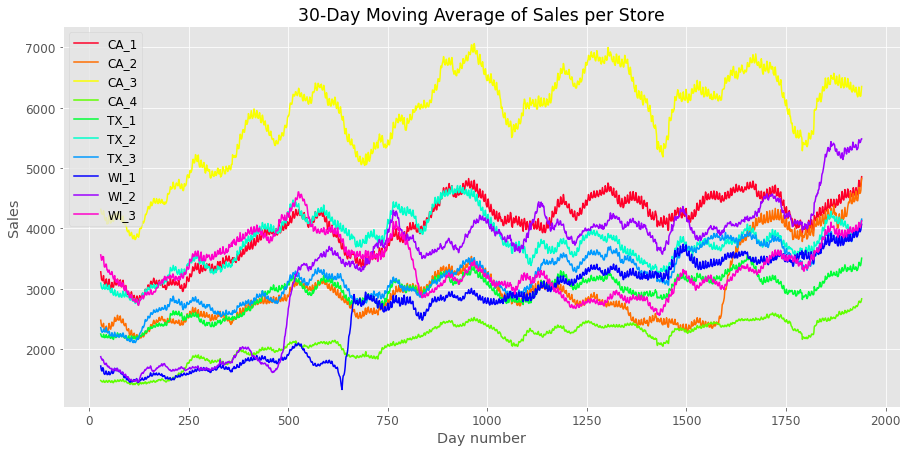
\includegraphics[width=0.98\textwidth]{figures/exploratory_data_analysis/store_sales.png}}
    \caption{30-day moving average of sales per store.}
    \label{fig:store_sales}
\end{figure} 


\section{Departments}
\begin{wrapfigure}{r}{0.55\textwidth}
    \vspace{-10pt}
    \centering
    \captionsetup{width=0.52\textwidth}
    \fbox{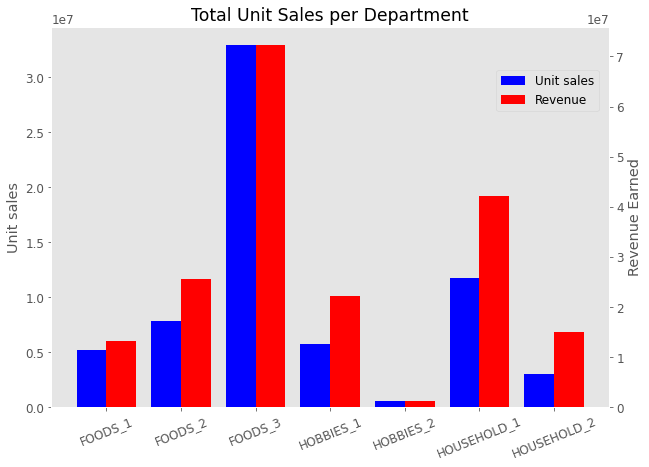
\includegraphics[width=0.52\textwidth]{figures/exploratory_data_analysis/sales_rev_depts.png}}
    \caption{Proportion of units sold and revenue earned per department.}
    \label{fig:sales_rev_depts}
    \vspace{-10pt}
\end{wrapfigure}
There are a total of seven departments in the dataset. 
There are three departments for the \texttt{FOODS} category, two departments for the \texttt{HOBBIES} category, and two departments for the \texttt{HOUSEHOLD} category.
The number of unit sales and revenue earned in each department is compared in Figure \ref{fig:sales_rev_depts}.
The bar chart shows that the \textit{FOODS\_3} department has the highest number of sales and revenue, followed by the \textit{HOUSEHOLD\_1} department.
Moreover, Figure \ref{fig:dept_sales} shows a 30-day moving average of the number of sales per department, which indicates that the \textit{FOODS\_3} department also has a higher volatility compared to the other departments.
\begin{figure}[H]
    \centering
    \fbox{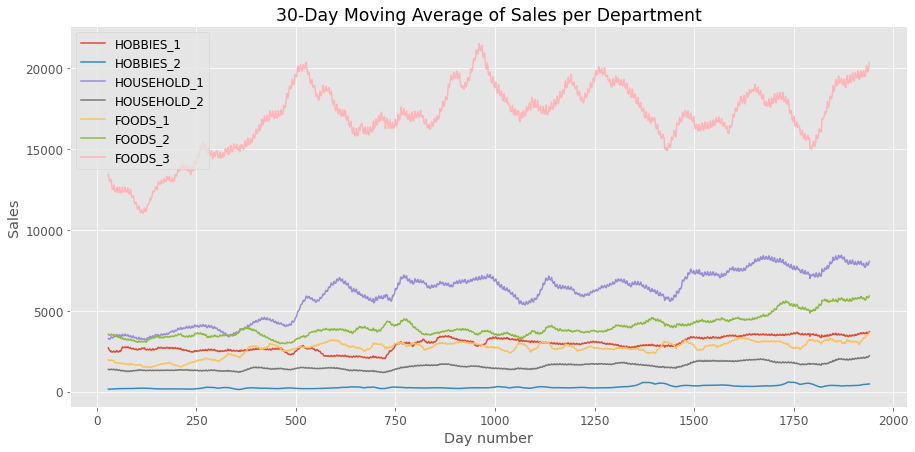
\includegraphics[width=0.98\textwidth]{figures/exploratory_data_analysis/dept_sales.png}}
    \caption{30-day moving average of sales per department.}
    \label{fig:dept_sales}
\end{figure}
